
% This LaTeX was auto-generated from MATLAB code.
% To make changes, update the MATLAB code and republish this document.

\documentclass{article}
\usepackage{graphicx}
\usepackage{color}

\sloppy
\definecolor{lightgray}{gray}{0.5}
\setlength{\parindent}{0pt}

\begin{document}

    
    
\section*{Assignment 2}

\begin{par}
Abhinav Moudgil
\end{par} \vspace{1em}
\begin{par}
201331039
\end{par} \vspace{1em}

\subsection*{Contents}

\begin{itemize}
\setlength{\itemsep}{-1ex}
   \item Convergence proof for single sample perceptron
   \item Single sample perceptron
   \item Single sample perceptron with margin
   \item Relaxation algorithm with margin
   \item Widrow-Hoff or Least Mean Squared (LMS) Rule
   \item Combined Plot
   \item Effect of initialization
   \item Effect of margin
   \item Neural network for handwritten digit classification
\end{itemize}


\subsection*{Convergence proof for single sample perceptron}

We need to show each iteration brings weight vector closer to solution region. Let the solution vector be \^{a}. 
\begin{par} 
$$ a(k+1) - \aplha \^{a} = (a(k) - \alpha \^{a}) + y^k $$ 
Taking norm and squaring,
$$ \|  a(k+1) - \aplha \^{a} \|^2 = \|  a(k) - \aplha \^{a} \|^2 + 2(a(k)  - \alpha \^{a}) ^ t y ^ k + \|y^k\|^2 $$ 

Since $y^k$ was misclassified, $a^t (k) y^k \leq 0$, thus 
$$ \|  a(k+1) - \aplha \^{a} \|^2 \leq \|  a(k) - \aplha \^{a} \|^2 + \|y^k\|^2 - 2 \alpha \^{a}^t y ^ k
 
After k corrections, 
$$ \|  a(k+1) - \aplha \^{a} \|^2 \leq \|  a(k) - \aplha \^{a} \|^2 - k \beta^2

where \beta^2 = max$\|y\|^2$

Hence, sequence of corrections must terminate after no more than $k_0$ corrections, where

$$ k_0 =  \frac{\|  a(1) - \aplha \^{a} \|^2}{\beta^2} $$ 

\end{par}

\subsection*{Single sample perceptron}

\begin{par}
Method:
\end{par} \vspace{1em}
\begin{par}
Weight vector for classification is updated each time we encounter a misclassified sample. This process is repeated over the training set until all samples are classified.
\end{par} \vspace{1em}
\begin{par}
Code:
\end{par} \vspace{1em}
\begin{verbatim}
clear;
clc;
close all;
tic

x = [1 7; 6 3; 7 8; 8 9; 4 5; 7 5; 3 1; 4 3; 2 4; 7 1; 1 3; 4 2];
y(:, 2 : 3) = x;
y(:, 1) = 1;

% Normalization of vector spaces
y(7 : 12, :) = -y(7 : 12, :);

%Weight vector initialization
a = [1 1 1];

% Perceptron function
g = @(a, y) a * y';

figure
s = scatter(y(1 : 6, 2), y(1 : 6, 3), 25, 'b', '*');
hold on;
t = scatter(-y(7 : 12, 2),-y(7 : 12, 3), 25, 'r', '+');

k = 0;
p = -2:0.01:10;
n = size(y, 1);
while nnz((a * y') > 0) ~= n
    k = mod(k, n) + 1;
    yk = y(k, :);
    if (g(a, yk) <= 0)
        a = a + yk;
    end
end

% Exceptional Handling for a(3) = 0 (Vertical line)
if (a(3) ~= 0)
    q = (- a(2) * p - a(1))/a(3);
    plot(p, q);
else
    hx = -a(1)/a(2) * ones(1, 10);
    hy = 1 : 10;
    plot(hx, hy);
end

toc
\end{verbatim}

        \color{lightgray} \begin{verbatim}Elapsed time is 0.061633 seconds.
\end{verbatim} \color{black}
    
\includegraphics [width=4in]{p2_01.eps}


\subsection*{Single sample perceptron with margin}

\begin{par}
Method:
\end{par} \vspace{1em}
\begin{par}
Single sample rule is followed along with margin 'b' make sure that points are not too close to decision boundry.
\end{par} \vspace{1em}
\begin{par}
Code:
\end{par} \vspace{1em}
\begin{verbatim}
tic

x = [1 7; 6 3; 7 8; 8 9; 4 5; 7 5; 3 1; 4 3; 2 4; 7 1; 1 3; 4 2];
y(:, 2 : 3) = x;
y(:, 1) = 1;

% Normalization of vector spaces
y(7 : 12, :) = -y(7 : 12, :);

%Weight vector initialization
a = [1 1 1];

% Margin
b = -100;

% Perceptron function
g = @(a, y) a * y' + b;

%figure
%s = scatter(y(1 : 6, 2), y(1 : 6, 3), 25, 'b', '*');
%hold on;
%t = scatter(-y(7 : 12, 2),-y(7 : 12, 3), 25, 'r', '+');

k = 0;
p = -2:0.01:10;
n = size(y, 1);
while nnz(g(a, y) > 0) ~= n
    k = mod(k, n) + 1;
    yk = y(k, :);
    if (g(a, yk) <= 0)
        a = a + yk;
    end

end

% Exceptional Handling for a(3) = 0 (Vertical line)
if (a(3) ~= 0)
    q = (- a(2) * p - a(1))/a(3);
    plot(p, q);
else
    hx = -a(1)/a(2) * ones(1, 10);
    hy = 1 : 10;
    plot(hx, hy);
end

toc
\end{verbatim}

        \color{lightgray} \begin{verbatim}Elapsed time is 0.627997 seconds.
\end{verbatim} \color{black}
    
\includegraphics [width=4in]{p2_02.eps}


\subsection*{Relaxation algorithm with margin}

\begin{par}
Method:
\end{par} \vspace{1em}
\begin{par}
Following perceptron criterion function Jp is chosen:
\end{par} \vspace{1em}
\begin{par}
$$ J_r(a) = \frac{1}{2} \sum_{y \in \gamma}^{} \frac{(a^t y - b)^2}{
\|y\|^2 } $$
\end{par} \vspace{1em}
\begin{par}
Its gradient is more continuous and smooth. Since longest sample vector can dominate the perceptron criterion function, hence normalization is done.
\end{par} \vspace{1em}
\begin{verbatim}
tic
x = [1 7; 6 3; 7 8; 8 9; 4 5; 7 5; 3 1; 4 3; 2 4; 7 1; 1 3; 4 2];
y(:, 2 : 3) = x;
y(:, 1) = 1;

% Normalization of vector spaces
y(7 : 12, :) = -y(7 : 12, :);

%Weight vector initialization
a = [1 1 1];

%Margin
b = 100;

% Perceptron function
g = @(a, y) a * y' - b;

%figure
%s = scatter(y(1 : 6, 2), y(1 : 6, 3), 25, 'b', '*');
%hold on;
%t = scatter(-y(7 : 12, 2),-y(7 : 12, 3), 25, 'r', '+');

k = 0;
p = -2:0.01:10;
n = size(y, 1);

eta = 2.1;
while nnz(g(a, y) > 0) ~= n
    k = mod(k, n) + 1;
    yk = y(k, :);
    if (g(a, yk) <= 0)
       a = a - ((eta * g(a, yk))/(norm(yk)^2)) * yk;
    end
end

% Exceptional Handling for a(3) = 0 (Vertical line)
if (a(3) ~= 0)
    q = (- a(2) * p - a(1))/a(3);
    plot(p, q);
else
    hx = -a(1)/a(2) * ones(1, 10);
    hy = 1 : 10;
    plot(hx, hy);
end

toc
\end{verbatim}

        \color{lightgray} \begin{verbatim}Elapsed time is 0.024712 seconds.
\end{verbatim} \color{black}
    
\includegraphics [width=4in]{p2_03.eps}


\subsection*{Widrow-Hoff or Least Mean Squared (LMS) Rule}

\begin{par}
Method:
\end{par} \vspace{1em}
\begin{par}
In this procedure, we consider all data samples rather than misclassified ones. Margin vector 'b' is taken. This procedure might not yield a seperating hyperplance but a reasonable one.
\end{par} \vspace{1em}
\begin{par}
Code:
\end{par} \vspace{1em}
\begin{verbatim}
tic

x = [1 7; 6 3; 7 8; 8 9; 4 5; 7 5; 3 1; 4 3; 2 4; 7 1; 1 3; 4 2];
y(:, 2 : 3) = x;
y(:, 1) = 1;

% Normalization of vector spaces
y(7 : 12, :) = -y(7 : 12, :);

%Weight vector initialization
a = [1 1 1];

%Margin
b = 10;

% Perceptron function
g = @(a, y) a * y' - b;
rownorm = @(x,p) sum(abs(x).^p,2).^(1/p);

%figure
%s = scatter(y(1 : 6, 2), y(1 : 6, 3), 25, 'b', '*');
%hold on;
%t = scatter(-y(7 : 12, 2),-y(7 : 12, 3), 25, 'r', '+');

k = 0;
p = -2:0.01:10;
n = size(y, 1);

theta = 1 * ones(12, 1);
eta = 0.5;
count = 1;
while nnz(rownorm(((eta/count) * repmat(g(a, y)', 1, 3) .* y), 2) < theta) ~= n
    k = mod(k, n) + 1;
    yk = y(k, :);
    a = a - ((eta/count) * g(a, yk)) * yk;
    count = count + 1;
end

% Exceptional Handling for a(3) = 0 (Vertical line)
if (a(3) ~= 0)
    q = (- a(2) * p - a(1))/a(3);
    plot(p, q);
else
    hx = -a(1)/a(2) * ones(1, 10);
    hy = 1 : 10;
    plot(hx, hy);
end

toc


hold off
\end{verbatim}

        \color{lightgray} \begin{verbatim}Elapsed time is 1.578698 seconds.
\end{verbatim} \color{black}
    
\includegraphics [width=4in]{p2_04.eps}


\subsection*{Combined Plot}

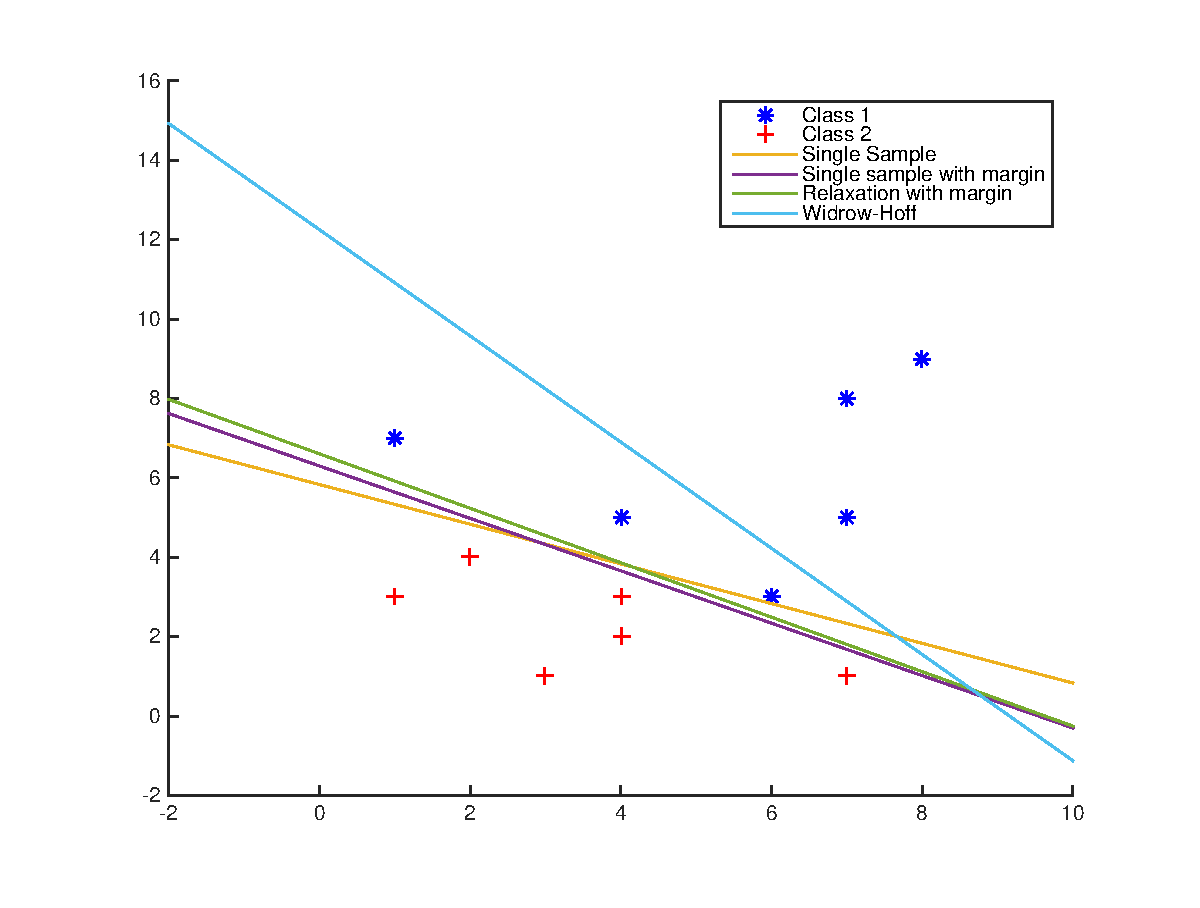
\includegraphics [width=4in]{plots.eps}

\subsection*{Effect of initialization}

\begin{par}
Weights are initialized randomly within a certain range. Average convergence time for certain ranges of weights are tabulated below: 
\end{par} \vspace{1em}
\begin{center}
\begin{tabular}{|p{3cm}||p{2cm}|p{2cm}|p{2cm}|p{2cm}|} \hline
\begin{par} Initial Weights Range\end{par} & \begin{par} Single sample\end{par} & \begin{par} Single sample with margin\end{par} & \begin{par} Relaxation with margin\end{par} & \begin{par} Widrow Hoff\end{par} \\ \hline
$[-1, 1]$ & 0.068177 & 0.570688 & 0.070865 & 9.170230\\
$[1000, 1000000]$ & 50.107077 & 17.411268 & 0.073862 & 30.43232 \\
$[0, 2]$ & 0.082015 & 0.568841 & 0.075528 &  6.448462\\
$[-100000, 100000]$ & 3.703376 & 6.654690 & 0.068799 & 20.32312\\ \hline
\end{tabular}
\end{center}

\begin{par}
Convergence time also depends on margin. Above convergence time are calculated with margin = 100. LMS has highest time of convergence in above table. It is not because of weight initialization. Initial value of learning and threshold for error also plays a very important role in convergence. In LMS, low threshold for error is set to yield maximum classification possible. 
\end{par}

\subsection*{Effect of margin}

\begin{par} 
\textbf{\textit{Singe sample with margin}} 


\vspace{1em}

\begin{center}
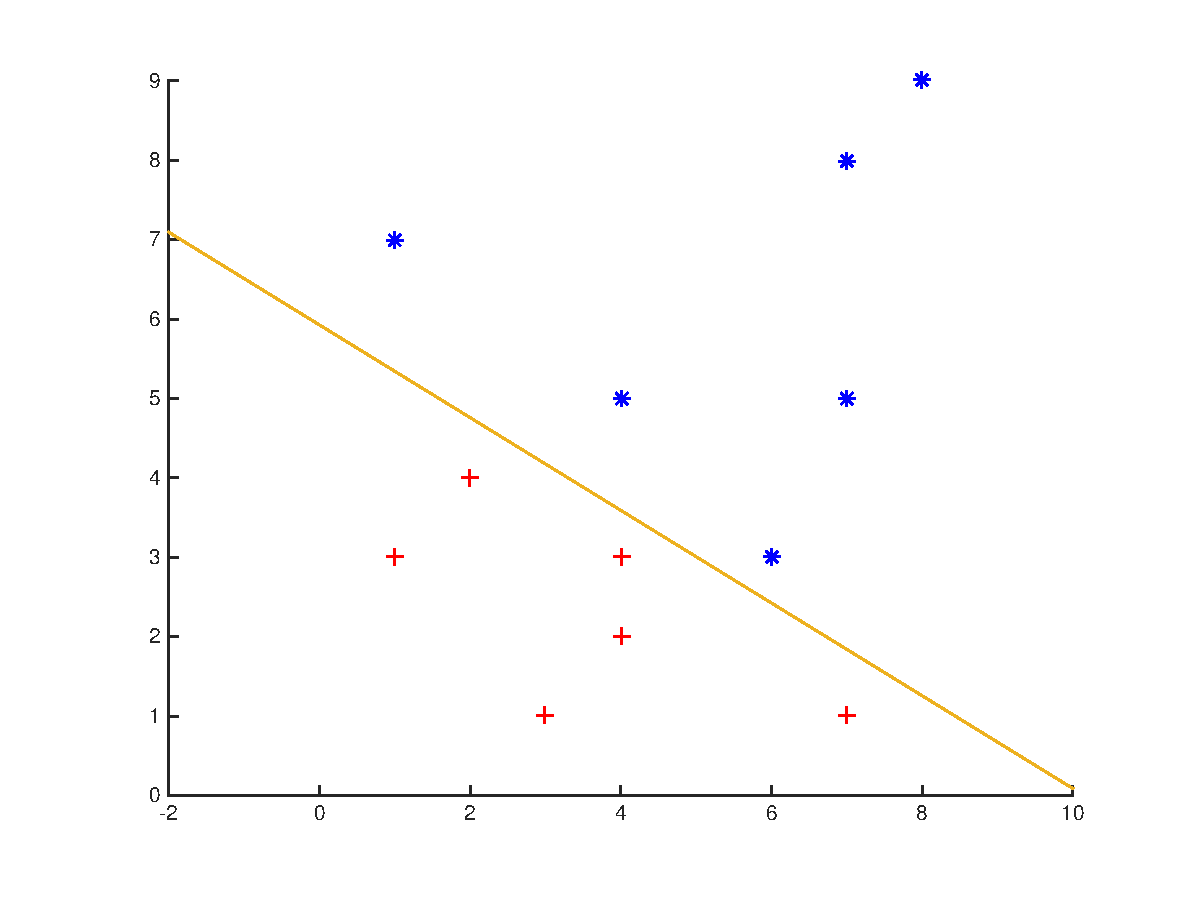
\includegraphics[width = 2in]{p2b5.eps}
\begin{par} {Margin = 5} \end{par}

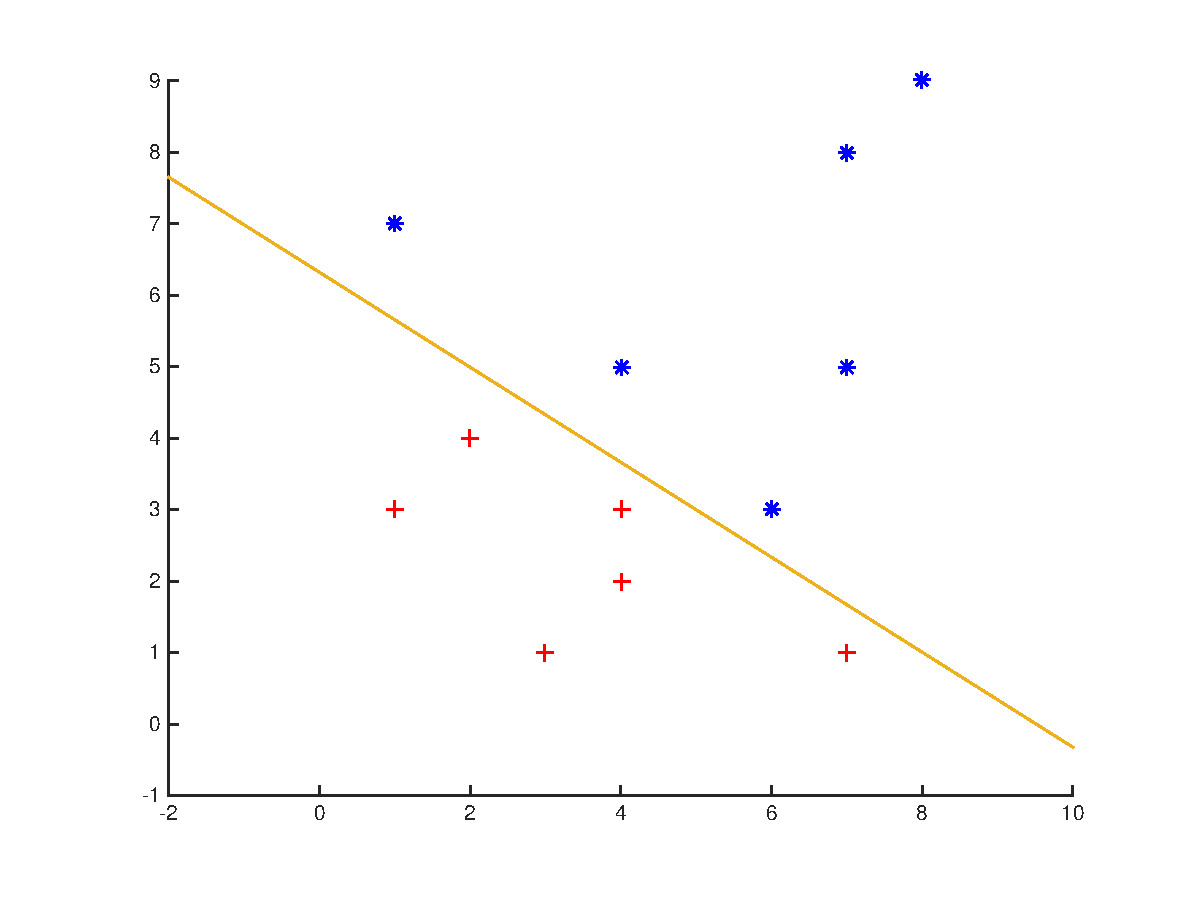
\includegraphics[width = 2in]{p2b100.eps}
\begin{par} {Margin = 100} \end{par}

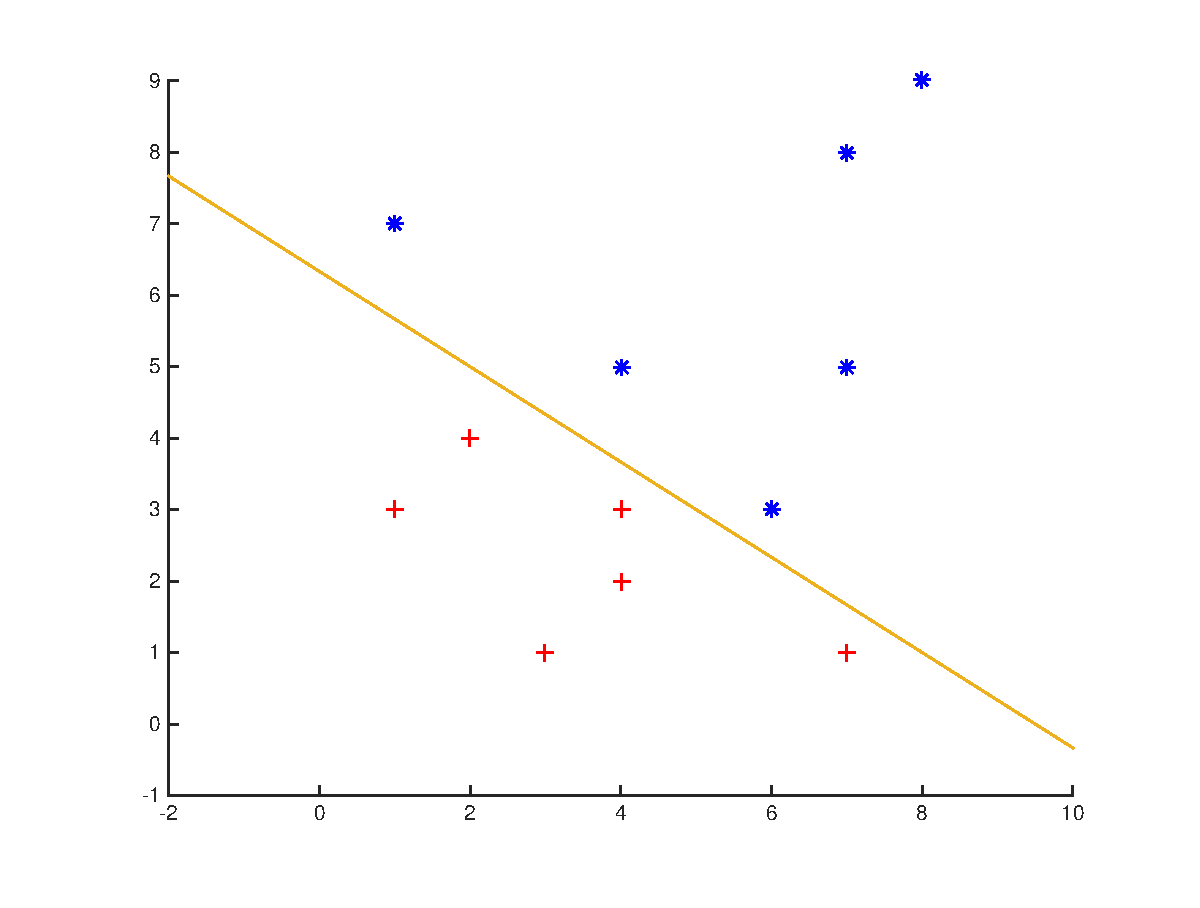
\includegraphics[width = 2in]{p2b1000.eps}
\begin{par} {Margin = 1000} \end{par}
\end{center}

\textbf{\textit{Relaxation with margin}} 

\vspace{1em}

\begin{center}
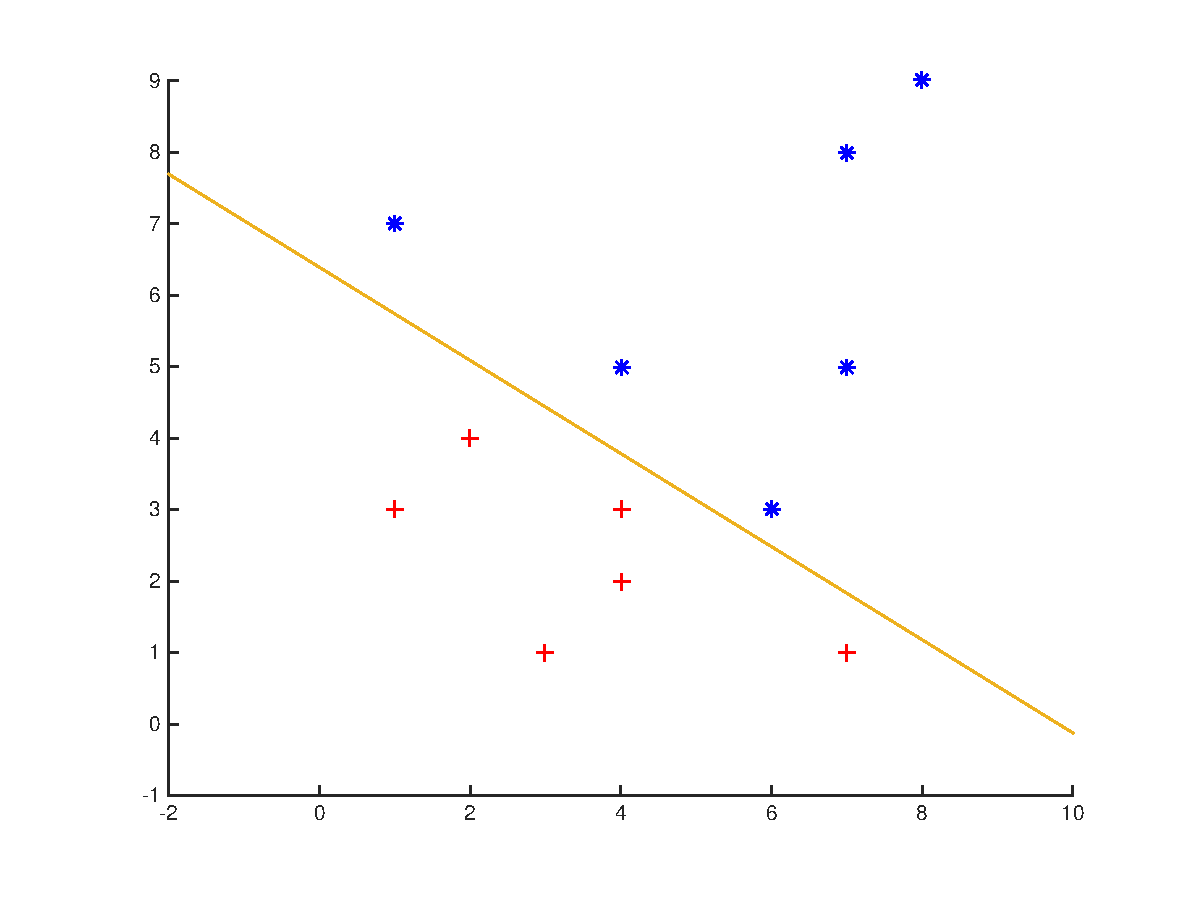
\includegraphics[width = 2in]{p2c5.eps}
\begin{par} {Margin = 5} \end{par}

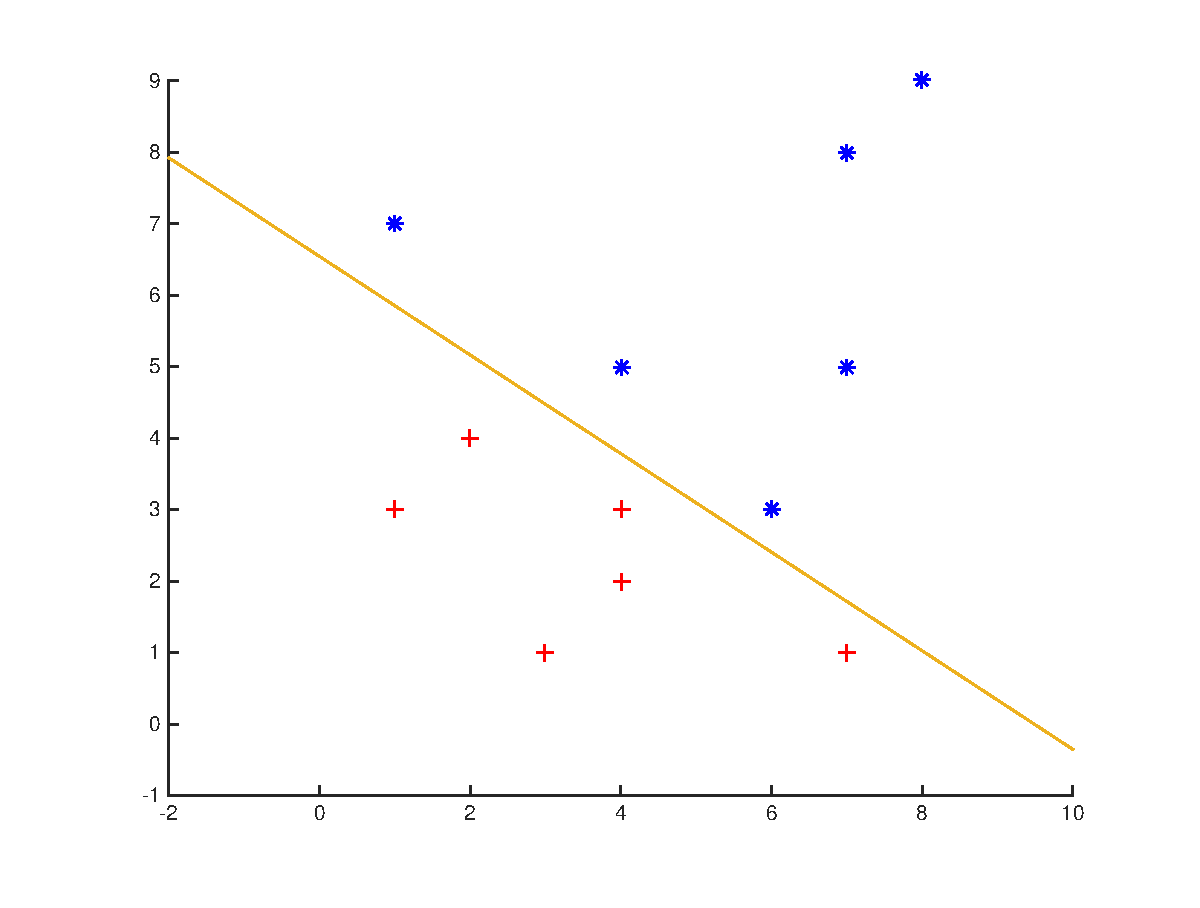
\includegraphics[width = 2in]{p2c100.eps}
\begin{par} {Margin = 100} \end{par}

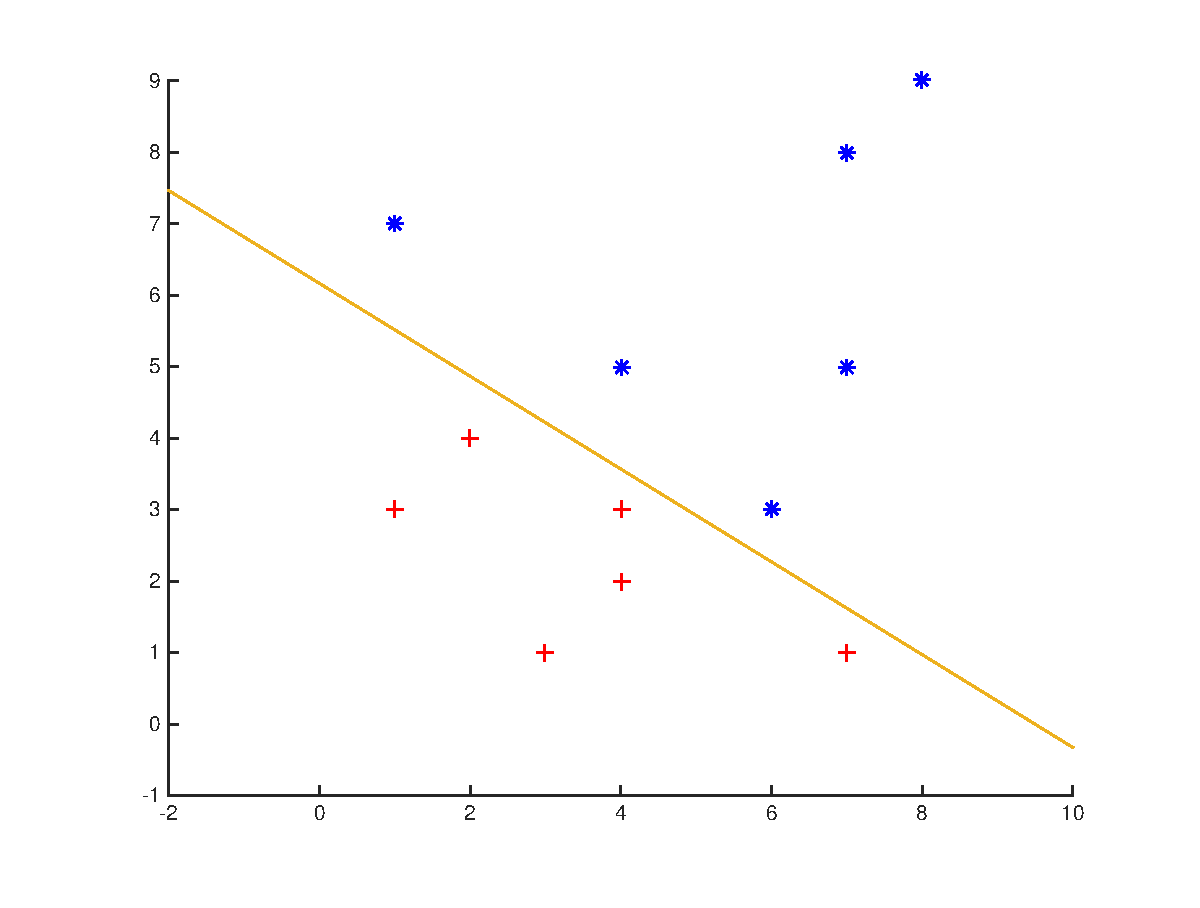
\includegraphics[width = 2in]{p2c1000.eps}
\begin{par} {Margin = 1000} \end{par}
\end{center}
\vspace{1em}
Following are the convergence time(in seconds) for both the algorithms: 
\vspace{1em}
\begin{center}
\begin{tabular}{|c|c|c|c|} \hline
\begin{par} Margin \end{par} & \begin{par} Single sample with margin\end{par} & \begin{par} Relaxation with margin\end{par} \\ \hline
5 & 0.126212 & 0.079206\\
100 & 0.570688 &  0.086744\\
1000 & 5.050803 & 0.095713\\ \hline
\end{tabular}
\end{center}

\end{par}

\subsection*{Neural network for handwritten digit classification}

\begin{par}
\textbf{Dataset}: Optical Recognition of Handwritten Digits Data Set \\ \\https://archive.ics.uci.edu/ml/datasets/Optical+Recognition+of+Handwritten+Digits 
\\ Dataset was trimmed to obtain only training and test samples of class 0 and 7. This was done using single bash command. 
\\ \\
\textbf{Preprocessing}: 32x32 bitmap images are processed to 8x8 data using by counting number of pixels in 4x4 blocks. Thus each sample contains 64 features and one class (0 or 7). 
\\ \\
\textbf{Classifier}:
\\
Optimal Model: 64-70-2 \\ 
Different number of hidden units were tested to obtain the most optimal model that has average accuracy of 99.72\% for this dataset. It also agrees with general rule of m/10 hidden units where m is the number of training samples. \\ 
Bias units are taken both at input and hidden layer. \\ 
Feed forward operation function: \\

\textbf{Code:}
\end{par}

\begin{verbatim}

%% Neural Network with one hidden layer
% Neural network for handwritten digit classification
% Model of neural network - 64-70-2

clear;
clc;
close all;

%% Training Phase
tic

filename = 'train.txt';
X = dlmread(filename, ',');
n = size(X, 1); % Number of training samples
t = X(:, size(X, 2));
%X = X(:, 1 : (size(X, 2) - 1));
X(:, size(X, 2)) = 1;
X = X';

% Initialization by feedforward operation
%bias1 = 1;
%bias2 = 1;
nHiddenUnits = 70;
f = @(x) logsig(x);
df = @(x) logsig(x) .* (1 - logsig(x));

a = -1/sqrt(size(X, 1));
b = 1/sqrt(size(X, 1));
wji = (b - a) .* rand(nHiddenUnits, size(X, 1)) + a;
netj = wji * X;

% Apply fnet from 1 : 32
yj(1 : nHiddenUnits - 1, :) = f(netj(1 : nHiddenUnits - 1, :));
yj(nHiddenUnits, :) = 1;
a = -1/sqrt(size(netj, 1));
b = 1/sqrt(size(netj, 1));
wkj = (b - a) .* rand(2, size(yj, 1)) + a;
netk = wkj * yj;
zk = f(netk);

% Backpropagation operation
tk(:, 1) = t < 6;
tk(:, 2) = t > 6;
tk = tk';
Jw = 0.5 * sum((tk - zk) .^ 2); % Gives error for each training sample in each column
delk = (tk - zk) .* df(netk);
delj = df(netj) .* (wkj' * delk);

eta = 1;
k = 0;
theta = 0.7;
while k < n
    k = mod(k, n) + 1; %Kth training sample
    xk = X(:, k);
    netj(:, k) = wji * X(:, k);
    yj(1 : nHiddenUnits - 1, k) = f(netj(1 : nHiddenUnits - 1, k));
    yj(nHiddenUnits, k) = 1;
    netk(:, k) = wkj * yj(:, k);
    zk(:, k) = f(netk(:, k));
    delk(:, k) = (tk(:, k) - zk(:, k)) .* df(netk(:, k));
    % delj(:, k) = df(netj(:, k)) * delk(:, k)' * wkj(:, k);
    delj(:, k) = df(netj(:, k)) .* (wkj' * delk(:, k));
    wkj = wkj + eta * delk(:, k) * yj(:, k)';
    wji = wji + eta * delj(:, k) * xk';
    
    % Updating all values according to new weights
    
    netj = wji * X;
    yj(1 : nHiddenUnits - 1, :) = f(netj(1 : nHiddenUnits - 1, :));
    yj(nHiddenUnits, :) = 1;
    netk = wkj * yj;
    zk = f(netk);
    
    % Error
    Jw(k) = 0.5 * sum((tk(:, k) - zk(:, k)) .^ 2);
end


%% Testing Phase


clear tk zk
filename = 'test.txt';
X = dlmread(filename, ',');
n = size(X, 1); % Number of test samples
t = X(:, size(X, 2));
% X = X(:, 1 : 64);
X(:, size(X, 2)) = 1;
X = X';
zk = zeros(2, size(X, 2));
tk(:, 1) = t < 6;
tk(:, 2) = t > 6;
tk = tk';
k = 0;

while k < n
    k = mod(k, n) + 1;
    xk = X(:, k);
    netj(:, k) = wji * X(:, k);
    yj(1 : nHiddenUnits - 1, k) = f(netj(1 : nHiddenUnits - 1, k));
    yj(nHiddenUnits, k) = 1;
    netk(:, k) = wkj * yj(:, k);
    zk(:, k) = f(netk(:, k));
end
zk = zk > 0.5;
err = tk - zk;
numberofErrors = sum(max(err ~= 0))
accuracy = (size(X, 2) - (numberofErrors))/size(X, 2)

toc

\end{verbatim}
\begin{par} 
\textbf{Observations:} \\
\\
1. Accuracy increases with increase in number of hidden units. But this might lead to over-fitting of data. \\
2. Without bias units, netj will have very high value, which implies yj (=f(netj)) will saturate to 1 if weights are positively initialized. Thus, f'(netj) will be 0 and weghts will not get updated. \\
3. Classification can also be done without bias units. Do normalization in each feature. This way, value of netj will never overshoot and we'll get average accuracy of around 99\%. \\ 
4. Convergence time increases with increase in number of hidden units. 
\end{par} 
\end{document}
    
